\subsubsection{Simulation of the $x_I$ and $y_I$ Controllers}
The final design for the $x_I$ and $y_I$ translational controllers is simulated in the following. The simulations are both of the translational velocity controller and the positioning controller. Simulations which are presented are of the controllers subjected to a step input reference signal and a corresponding simulation showing the related control action of each controller. 

In \autoref{fig:velocityControllersXY} the translational velocity controllers, $\dot{x}_I$ and $\dot{y}_I$, is subjected to a step input reference signal of \SI{1}{m s^{-1}} at \SI{0.5}{s} and \SI{2.5}{s}. This yields a settling time of \SI{6}{s} at an error band of 5 percent and an overshoot of 15 percent for both the $\dot{x}_I$ and $\dot{y}_I$. In \autoref{fig:velocityControllersXYAction} the corresponding control action for this step input reference signal is shown, both the needed an the actual.

\begin{minipage}{\linewidth}
    \begin{minipage}{0.5\linewidth}
        \begin{figure}[H]
            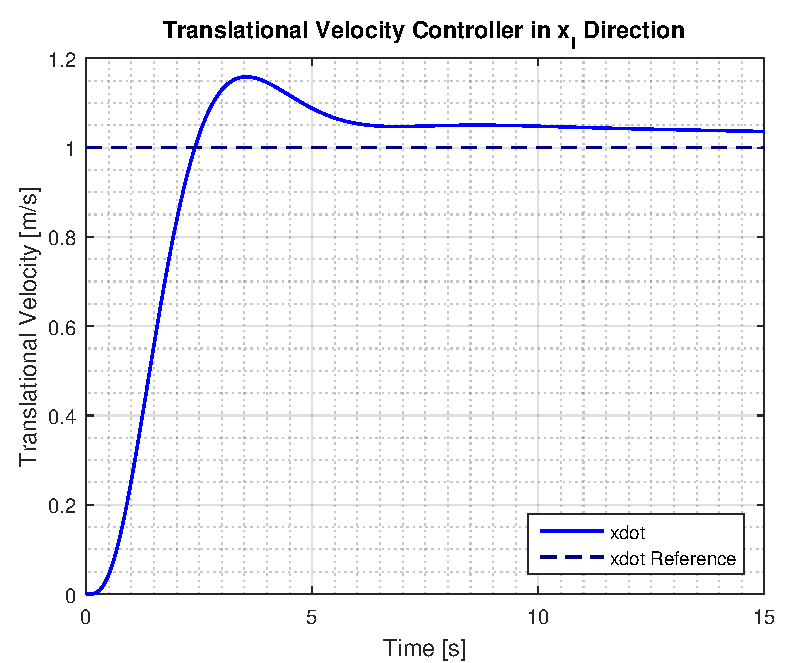
\includegraphics[scale=.58]{figures/velocityControllersXY}
            \centering			
            \captionof{figure}{A step response of the translational velocity controllers in $\dot{x}_I$ and $\dot{y}_I$. Both $\dot{x}_I$ and $\dot{y}_I$ is subjected to a step input reference signal of \SI{1}{m s^{-1}}. $\dot{x}_I$ at \SI{0.5}{s} and $y_I$ at \SI{2.5}{s}.}
            \label{fig:velocityControllersXY}
        \end{figure}
    \end{minipage}
    \hspace{0.03\linewidth}
    \begin{minipage}{0.5\linewidth}
        \begin{figure}[H]
            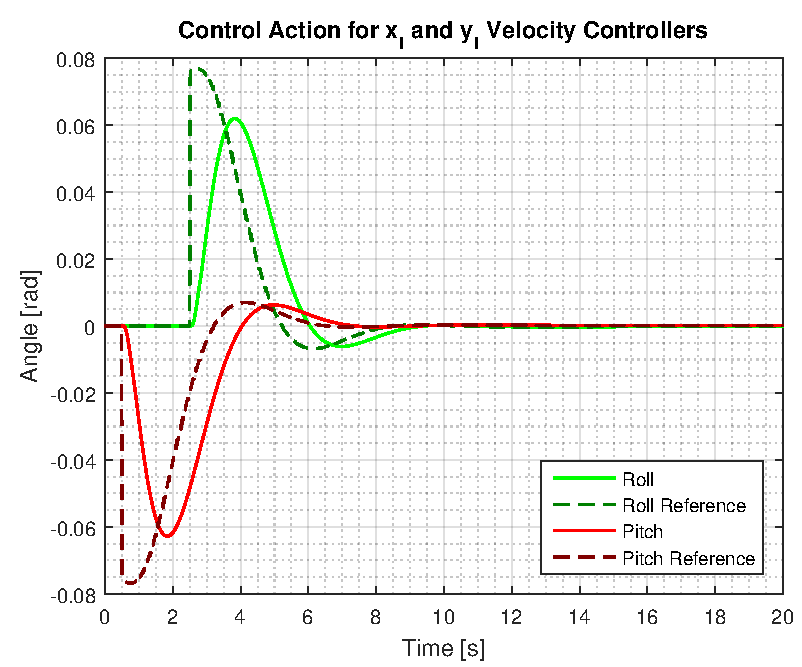
\includegraphics[scale=.58]{figures/velocityControllersXYAction}
            \centering
            \captionof{figure}{The actual control action for the actual performed step input together with the required control action needed to achieve the set step input from \autoref{fig:velocityControllersXY}.}
            \label{fig:velocityControllersXYAction}
        \end{figure}
    \end{minipage}
\end{minipage}

In \autoref{fig:positionControllersXY} the translational velocity controllers, $x_I$ and $y_I$, is subjected to a step input reference signal of \SI{1}{m s^{-1}} at \SI{0.5}{s} and \SI{2.5}{s}. Yielding a settling time of \SI{5}{s} at an error band of 5 percent and a overshoot of 2 percent for both the $x_I$ and $y_I$. As the position controllers are designed to have a closed loop bandwidth which is three times lower than the velocity bandwidth, a larger settling time is expected. However, as the overshoot is small compared to the velocity controller and the settling time has an error band of 5 percent, the settling time becomes lower.

\begin{minipage}{\linewidth}
    \begin{minipage}{0.46\linewidth}
        \begin{figure}[H]
            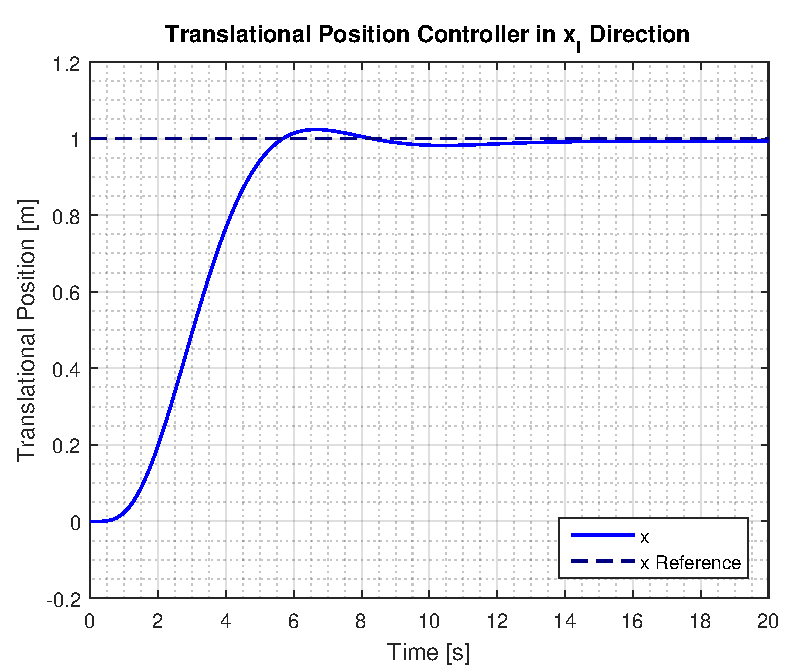
\includegraphics[scale=.61]{figures/positionControllersXY}
            \centering			
            \captionof{figure}{A step response of the position controllers in $x_I$ and $y_I$. Both $x_I$ and $y_I$ is subjected to a step input reference signal of \SI{1}{m s^{-1}}. $x_I$ at \SI{0.5}{s} and $y_I$ at \SI{2.5}{s}.}
            \label{fig:positionControllersXY}
        \end{figure}
    \end{minipage}
    \hspace{0.03\linewidth}
    \begin{minipage}{0.46\linewidth}
        \begin{figure}[H]
            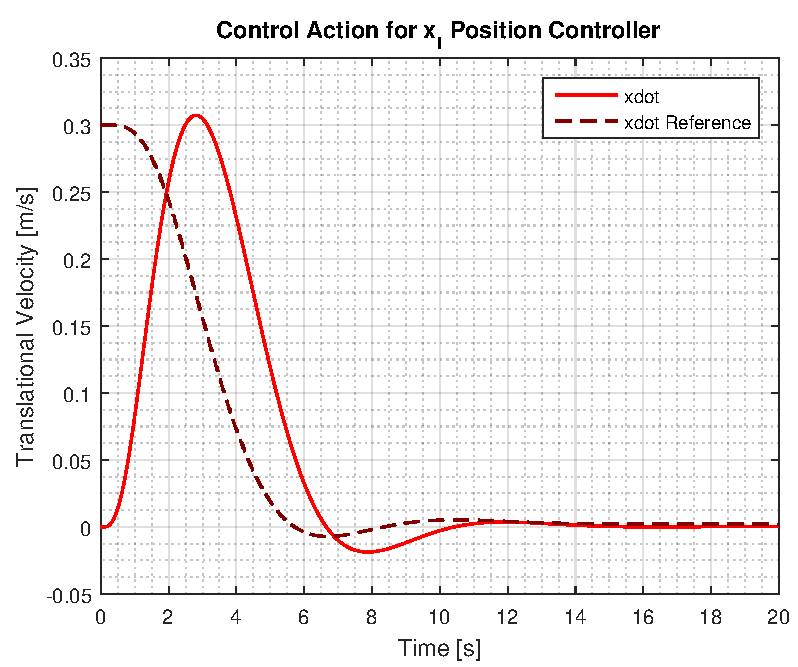
\includegraphics[scale=.61]{figures/positionControllersXYAction}
            \centering
            \captionof{figure}{The actual control action for the actual performed step  together with the required control action needed to achieve the set step reference from \autoref{fig:positionControllersXY}.}
            \label{fig:positionControllersXYAction}
        \end{figure}
    \end{minipage}
\end{minipage}

The controllers for the translational velocity and positioning in $x_I$ and $y_I$ have now been designed and simulated, the z controller can thereby be designed in the following section.
